\documentclass[slug=GL, room=HZDR\ Dresden/Rossendorf\,\ Geb.\ 620/123, supervisor=Martin\ Rehwald;\, Tim\ Ziegler]{../../Lab_Report_LaTeX/lab_report}

\title{Gaslaser}
\author{Oliver Matthes, Valentin Boettcher}
\usepackage[version=4]{mhchem}
\usepackage{todonotes}
\graphicspath{ {figs/} }
\newcommand{\laser}{\textsc{Laser}}

\newtheorem{acro}{Acronym}[section]
\begin{document}
\maketitle

\section{Einleitung}%
\label{sec:intro}
Der \laser{} ist seit seiner Erfindung in den 1960er Jahren in der
modernen Physik zu einem Standardwerkzeug geworden. Unter anderem
kann ein Laserstrahl zur Erzeugung von sehr tiefen Temperaturen
(Untersuchung von Quanteneffekten, Bose-Einstein Kondensation), zur
Erzeugung und Untersuchung von Schockwellen und zur Beschleunigung von
Elementarteilchen genutzt werden.

\todo{erlautern} Auch in der Technik findet der \laser{} aufgrund
der hohen Koh\"arenz und Intensit\"t des emmitierten Lichtstrahls
vielfach Anwendung. So hat man allt\"aglich mit auf Lasertechnologie
basierenden Barcode Scannern und CD-Spielern zu tun. Auch die moderne
Telekommunikationstechnik um das Internet nutzt \laser{} zur
Daten\"ubertragung.

Zum n\"aheren Verst\"andnis sollte zun\"achst das Akronym \laser{}
gekl\"art werden.

\begin{acro}[Laser]
\textsc{Light Amplification by Stimulated Emission of Radiation.}
\end{acro}

Dementsprechend verst\"arkt ein \laser{} also Licht durch Stimulierte
Emmision. Da die Stimulierte Emission von Strahlung ein Photon in
allen seinen Eigenschaften kopiert, wird im Allgemeinen koh\"arentes
und bedingt durch die Verst\"arkung sehr intesives Licht erzeugt.

Der grundlegende Aufbau eines Lasers ist erstaunlich einfach. So
besteht ein Laser aus:

\begin{enumerate}
\item einem aktiven Medium (Gase, Festk\"rper)
\item einem optischen Resonator (meist rotationssymmetrische, sph\"arische Spiegel)
\item einer ``Energiepumpe'' (Lichtblitze, Elektronenst\"osse)
\end{enumerate}

\begin{figure}[H]\centering\label{fig:aufb}
  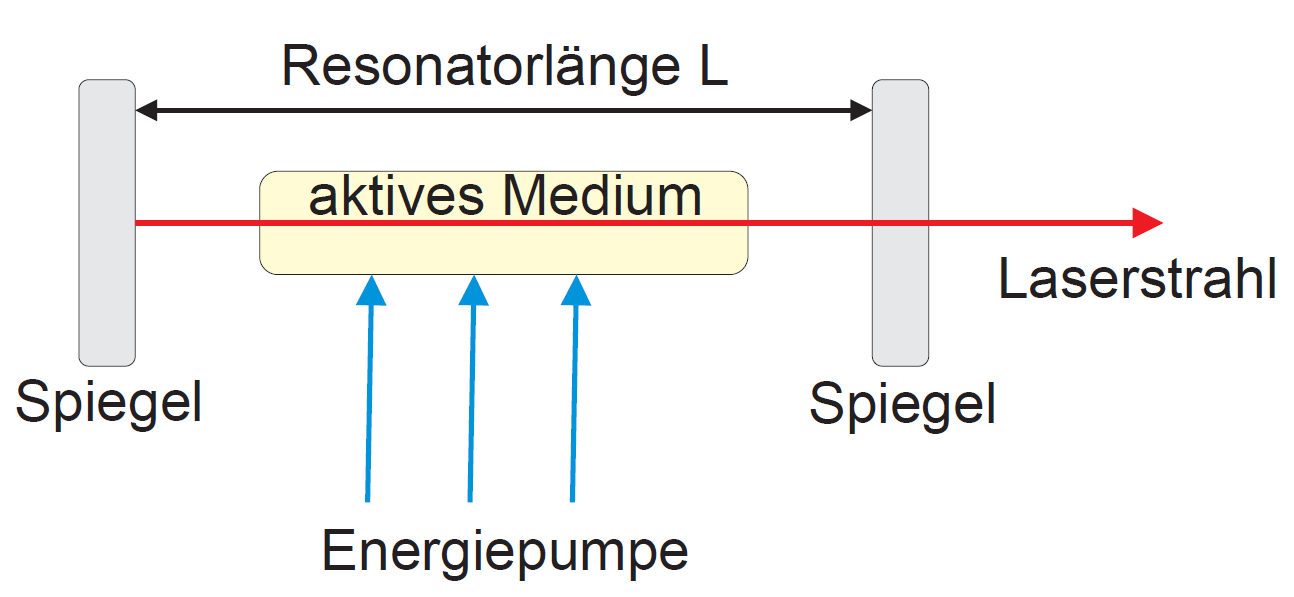
\includegraphics[width=.5\columnwidth]{schema.png}
  \caption[Aufbau]{Schema eines Lasers}
\end{figure}

Die Energiepumpe erzeugt im aktiven Medium eine
Ungleichgewichtsbesetzung von Energiniveaus, die die induzierte
Emission beg\"unstigt. Die Photonen oszillieren im Resonator mehrfach
und werden bei jedem Durchlauf verst\"arkt, bis sie den
Resonator verlassen.

\section{Theoretische Grundlagen}%
\label{sec:theo}

\subsection{Besetzungsinversion und Laserbedingung}%
\label{sec:inv}

Die Elektronen in Atomen nehmen nach der Quantenmechanik nur diskrete
Energien an. Wenn ein Elektron seinen Zustand wechselt, wird bei
diesem \"Ubergang Licht emmitiert oder absorbiert wobei f\"ur die
Energien \(E_i\) und die Frequenz des beteiligten Photons \(\nu\) gilt:

\begin{equation}
  \label{eq:transfreq}
  h\nu = E_2 - E_1
\end{equation}

Es gibt drei Prozesse, die nun die Anzahl der Atome im Grundzustand
\(N_1\) und der angeregten Atome \(N_2\) beeinflussen.

\begin{description}
\item[Absorbtion] Ein photon wird von einem Atom absorbiert, welches
  dementsprechend angeregt wird. Die H\"aufigkeit dieses Prozesses ist
  proportional zur spektralen Energiedichte.
\item[Spontane Emission] Ein angeregtes Atom geht in einen tieferen
  Zustand \"uber und sendet ein Photon aus. Dieser Prozess ist
  unabh\"angig von der umgebenden spektralen Energiedichte.
\item[Stimulierte Emission] Das Atom wird von einem passenden Photon
  zur Emmission eines zweiten, identischen Photons angeregt und geht
  in einen tieferen Zustand \"uber. Die H\"aufigkeit dieses Prozesses ist
  proportional zur spektralen Energiedichte.
\end{description}

Durch aufstellung von Ratengleichungen f\"ur das thermische
Gleichgewicht in einem Zweiniveausystem wird deutlich, dass in einem
solchen Fall die Spontane Emmission \"uberwiegt und keine
Verst\"arkung auftreten kann, da die Warscheinlichkeit f\"ur Absorbion
und Stimulierte Emmision gleich, sowie immer mehr Teilchen im
Grundzustand als im angeregten Zustand sind.

F\"ur die Photonenzahldichte \(q\) gilt mit der spektralen
Energiedichte \(\rho(\nu)\) und dem Einsteinkoeffizienten f\"ur
Stimulierte Emission und unter Vernachl\"assigung der spontanen
Emission:

\begin{equation}
  \label{eq:qrate}
  \dv{q}{t}=\rho(\nu)B_{21}(N_2-N_1)
\end{equation}

Damit eine Verst\"arkung auftritt muss gelten:

\begin{equation}
  \label{eq:first}
  \tag{Erste Laserbedingung}
  N_2>N_1
\end{equation}
\end{document}
